\begin{figure}[H]
\centering
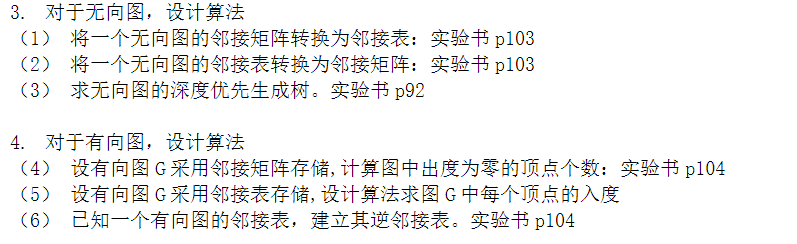
\includegraphics[width=\textwidth]{1-实验报告11-2025052622.png}
% \caption{}
\label{}
\end{figure}

\section{3}

\begin{figure}[H]
\centering
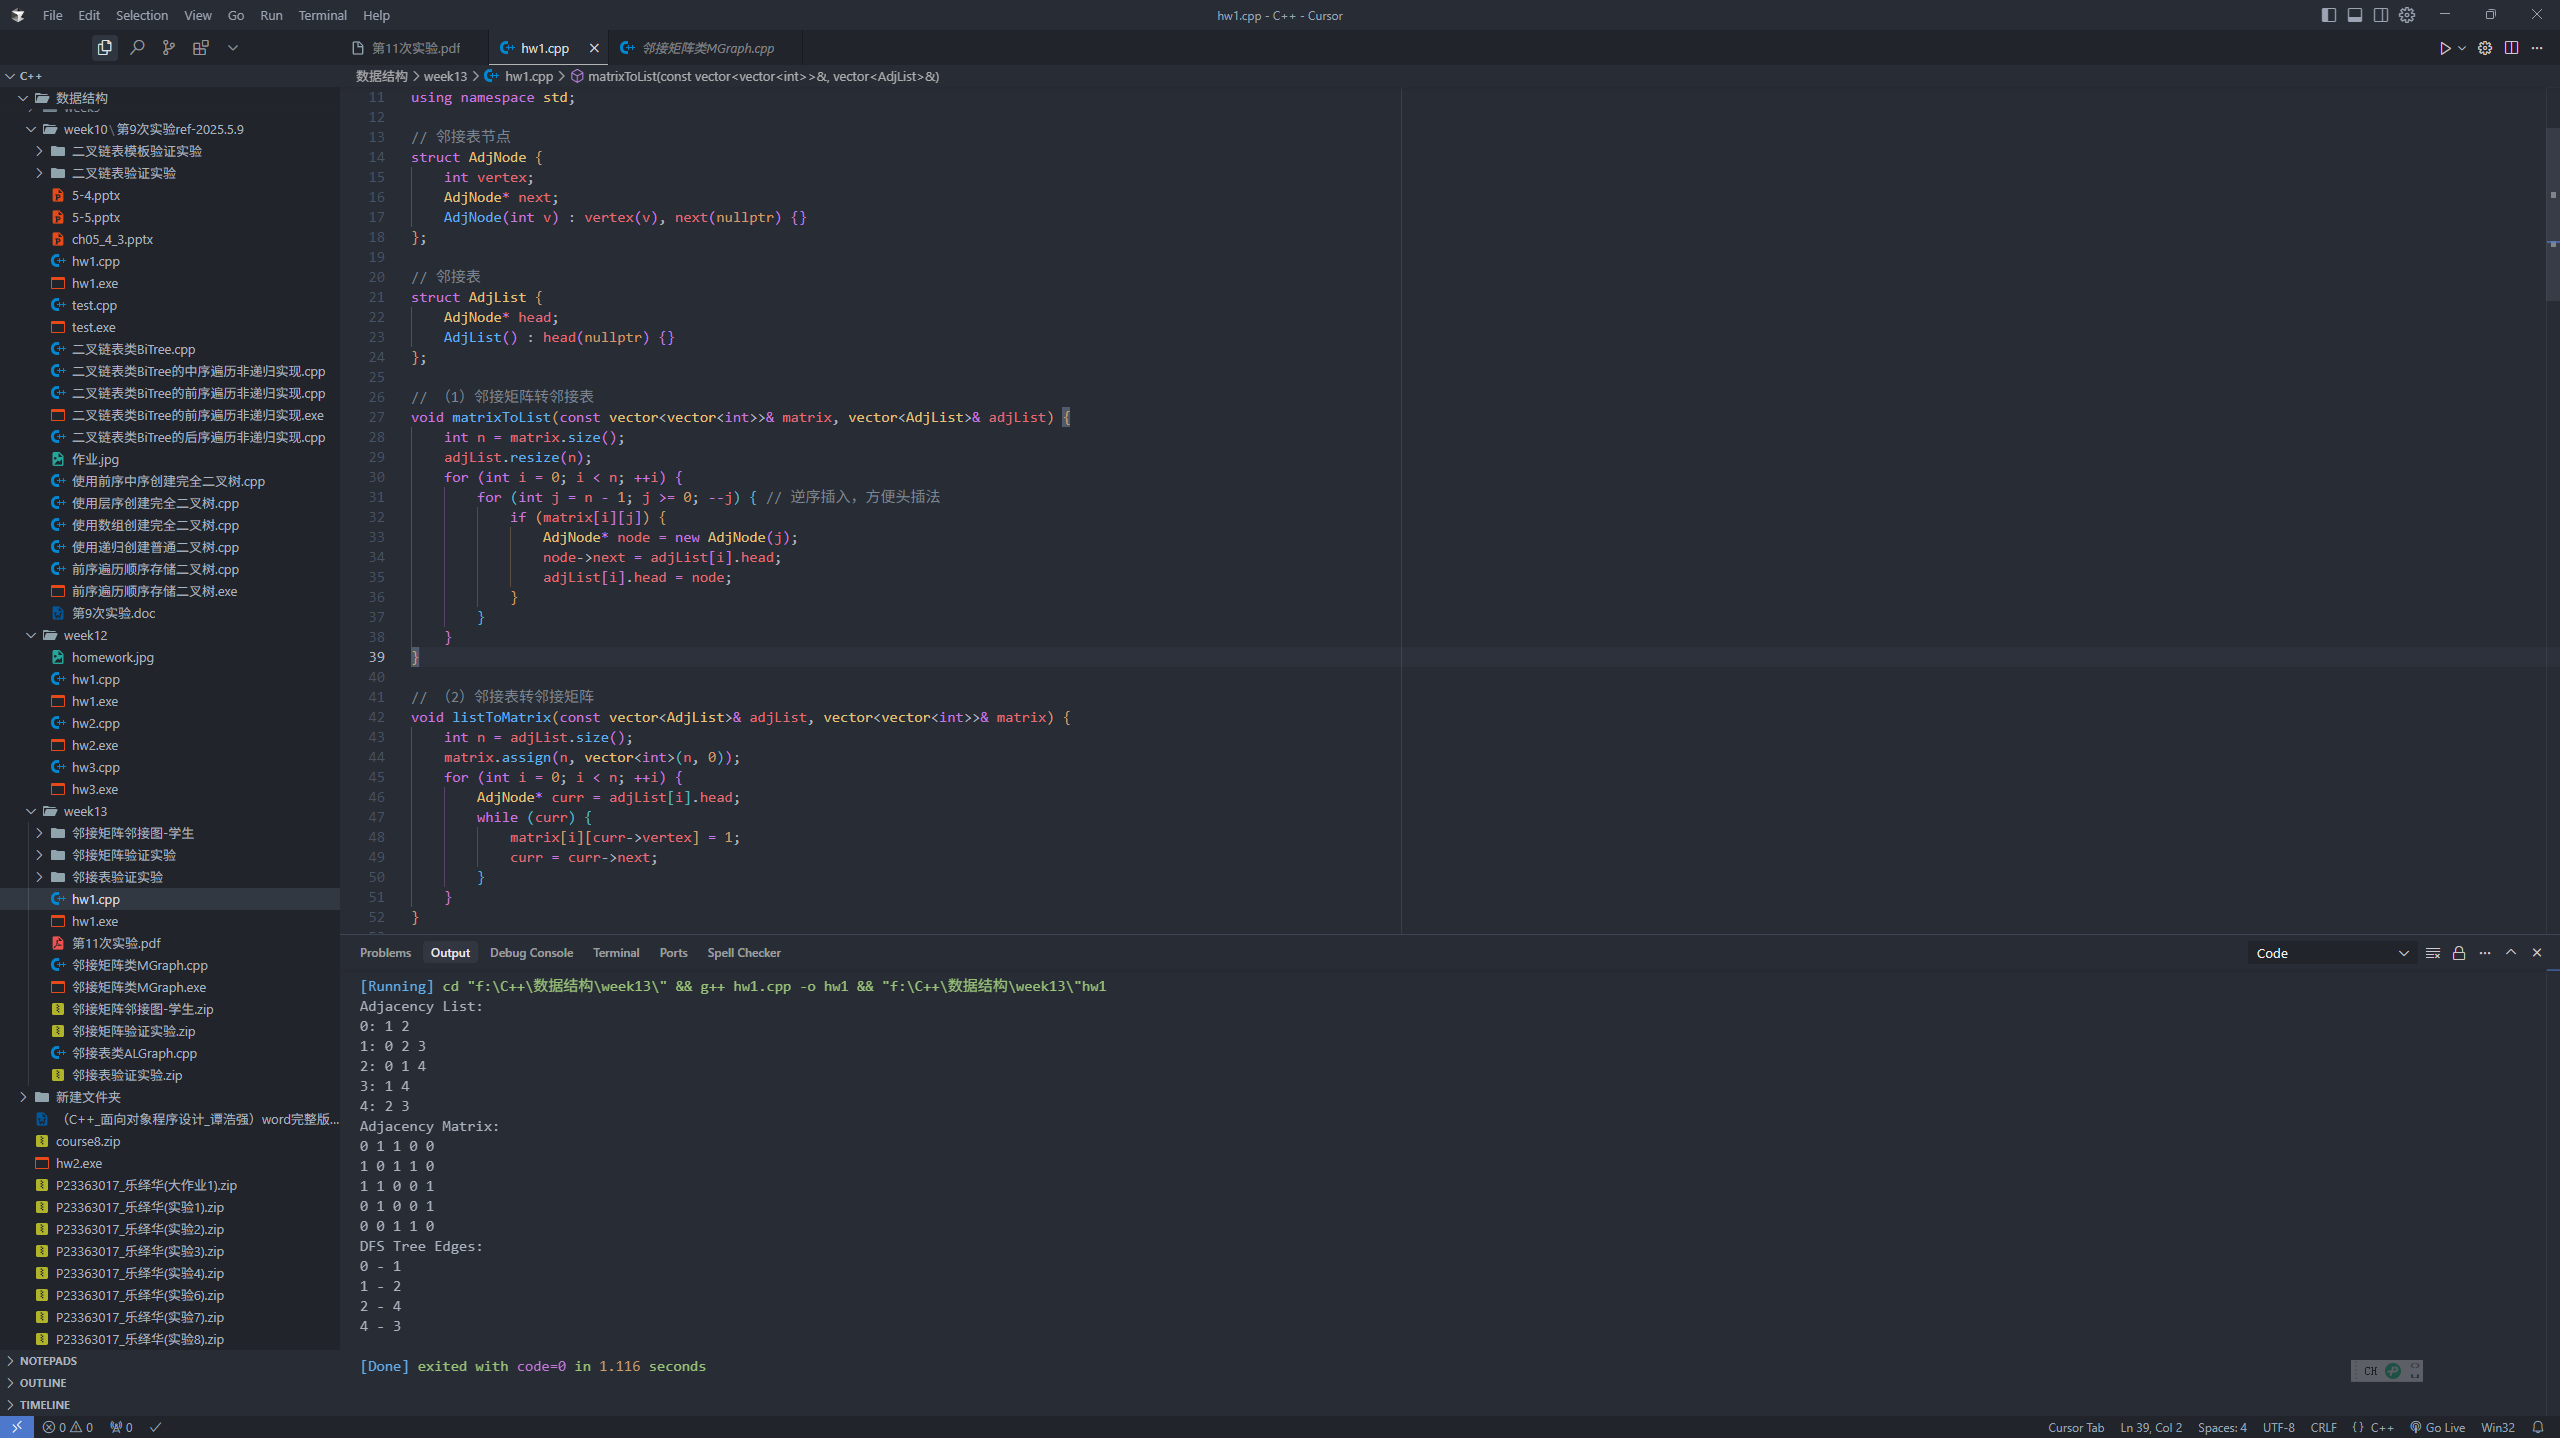
\includegraphics[width=\textwidth]{实验报告11-2025052622.png}
% \caption{}
\label{}
\end{figure}

\begin{lstlisting}[language=C++]
// 3. 针对无向图,设计如下算法:

// (1)将无向图的邻接矩阵转换为邻接表(参考实验书第103页)

// (2)将无向图的邻接表转换为邻接矩阵(参考实验书第103页)

// (3)求无向图的深度优先生成树(参考实验书第92页)

  
  
  

#include <iostream>

#include <vector>

#include <stack>

using namespace std;

  

// 邻接表节点

struct AdjNode {

    int vertex;

    AdjNode* next;

    AdjNode(int v) : vertex(v), next(nullptr) {}

};

  

// 邻接表

struct AdjList {

    AdjNode* head;

    AdjList() : head(nullptr) {}

};

  

// (1)邻接矩阵转邻接表

void matrixToList(const vector<vector<int>>& matrix, vector<AdjList>& adjList) {

    int n = matrix.size();

    adjList.resize(n);

    for (int i = 0; i < n; ++i) {

        for (int j = n - 1; j >= 0; --j) { // 逆序插入,方便头插法

            if (matrix[i][j]) {

                AdjNode* node = new AdjNode(j);

                node->next = adjList[i].head;

                adjList[i].head = node;

            }

        }

    }

}

  

// (2)邻接表转邻接矩阵

void listToMatrix(const vector<AdjList>& adjList, vector<vector<int>>& matrix) {

    int n = adjList.size();

    matrix.assign(n, vector<int>(n, 0));

    for (int i = 0; i < n; ++i) {

        AdjNode* curr = adjList[i].head;

        while (curr) {

            matrix[i][curr->vertex] = 1;

            curr = curr->next;

        }

    }

}

  

// (3)求无向图的深度优先生成树(DFS生成树)

void DFSUtil(int u, vector<AdjList>& adjList, vector<bool>& visited, vector<pair<int, int>>& treeEdges) {

    visited[u] = true;

    AdjNode* curr = adjList[u].head;

    while (curr) {

        int v = curr->vertex;

        if (!visited[v]) {

            treeEdges.push_back({u, v});

            DFSUtil(v, adjList, visited, treeEdges);

        }

        curr = curr->next;

    }

}

  

vector<pair<int, int>> DFSTree(vector<AdjList>& adjList) {

    int n = adjList.size();

    vector<bool> visited(n, false);

    vector<pair<int, int>> treeEdges;

    for (int i = 0; i < n; ++i) {

        if (!visited[i]) {

            DFSUtil(i, adjList, visited, treeEdges);

        }

    }

    return treeEdges;

}

  

// 辅助函数:打印邻接表

void printAdjList(const vector<AdjList>& adjList) {

    for (int i = 0; i < adjList.size(); ++i) {

        cout << i << ":";

        AdjNode* curr = adjList[i].head;

        while (curr) {

            cout << " " << curr->vertex;

            curr = curr->next;

        }

        cout << endl;

    }

}

  

// 辅助函数:打印邻接矩阵

void printMatrix(const vector<vector<int>>& matrix) {

    for (const auto& row : matrix) {

        for (int val : row) {

            cout << val << " ";

        }

        cout << endl;

    }

}

  

// 辅助函数:打印DFS生成树的边

void printDFSTree(const vector<pair<int, int>>& treeEdges) {

    cout << "DFS Tree Edges:" << endl;

    for (const auto& edge : treeEdges) {

        cout << edge.first << " - " << edge.second << endl;

    }

}

  

// 示例主函数

int main() {

  

    // The graph structure:

    //

    //      0

    //     / \

    //    1---2

    //    |   |

    //    3---4

    //

    // Adjacency matrix for reference:

    vector<vector<int>> matrix = {

        {0,1,1,0,0},

        {1,0,1,1,0},

        {1,1,0,0,1},

        {0,1,0,0,1},

        {0,0,1,1,0}

    };

  

    // 1. 邻接矩阵转邻接表

    vector<AdjList> adjList;

    matrixToList(matrix, adjList);

    cout << "Adjacency List:" << endl;

    printAdjList(adjList);

  

    // 2. 邻接表转邻接矩阵

    vector<vector<int>> matrix2;

    listToMatrix(adjList, matrix2);

    cout << "Adjacency Matrix:" << endl;

    printMatrix(matrix2);

  

    // 3. 求DFS生成树

    vector<pair<int, int>> treeEdges = DFSTree(adjList);

    printDFSTree(treeEdges);

  

    // 释放邻接表内存

    for (auto& list : adjList) {

        AdjNode* curr = list.head;

        while (curr) {

            AdjNode* tmp = curr;

            curr = curr->next;

            delete tmp;

        }

    }

  

    return 0;

}
\end{lstlisting}
\section{4}

\begin{figure}[H]
\centering
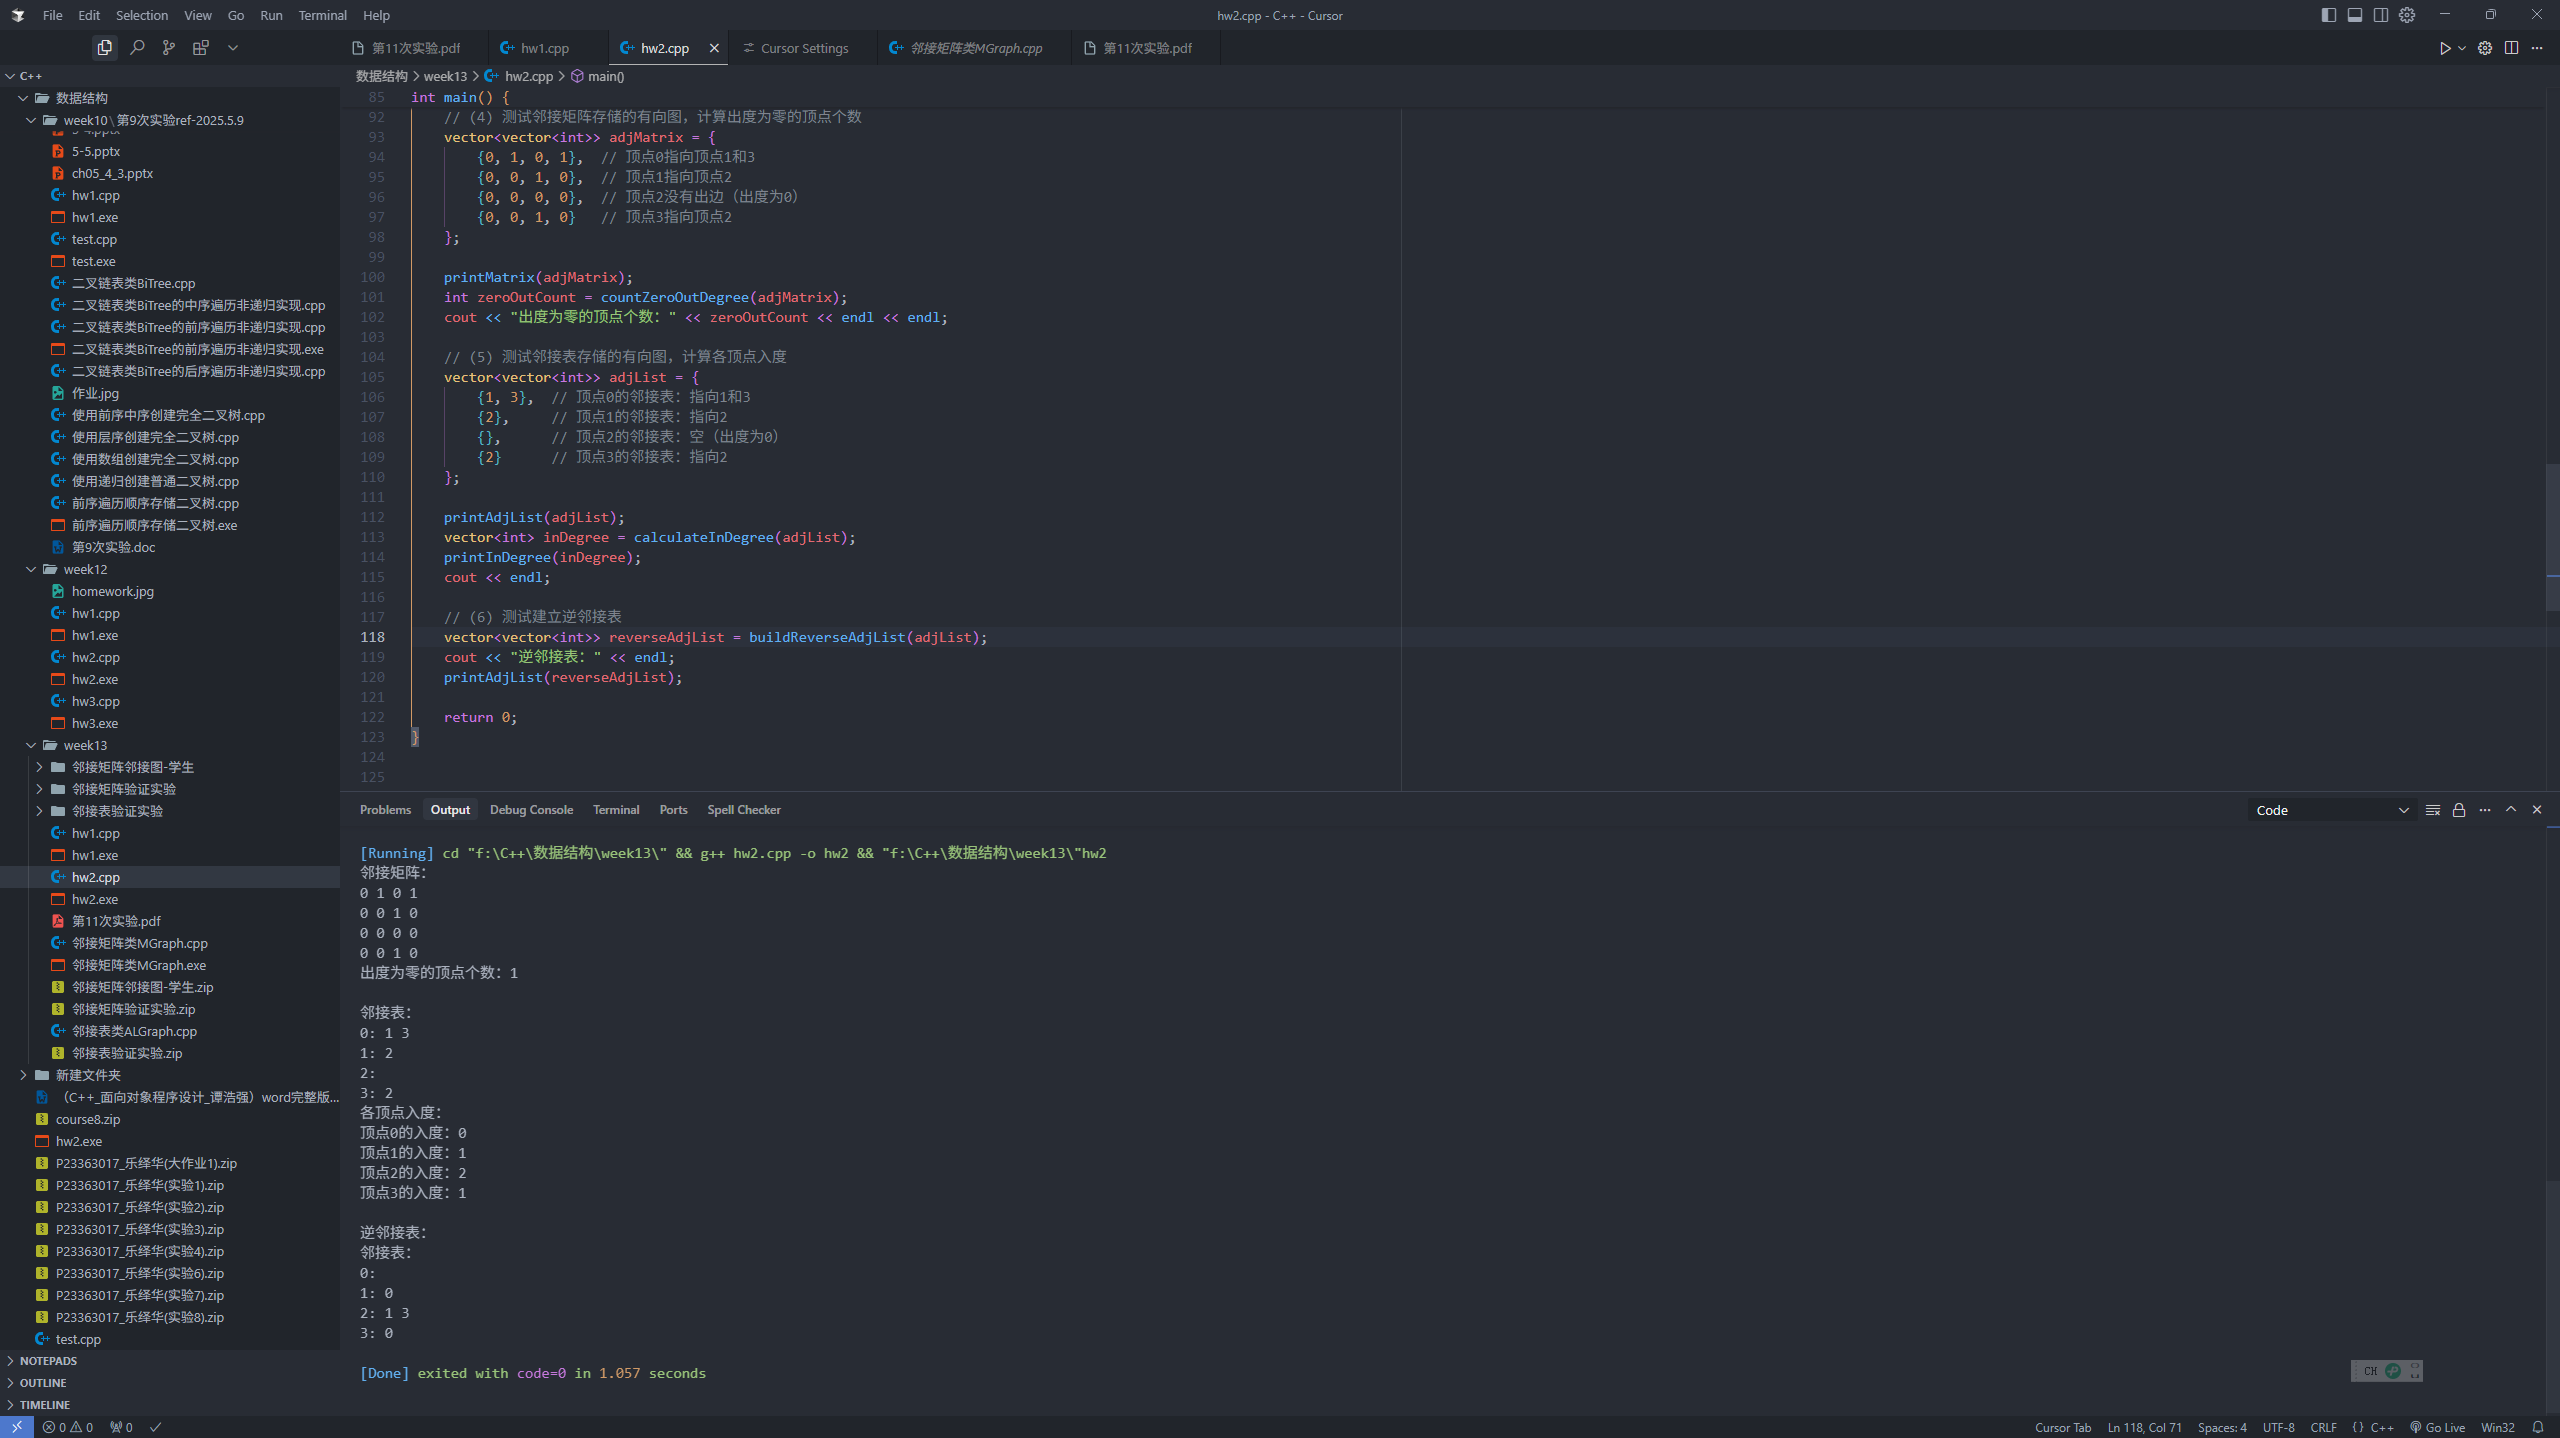
\includegraphics[width=\textwidth]{实验报告11-2025052623.png}
% \caption{}
\label{}
\end{figure}

\begin{lstlisting}[language=C++]
// 4. 对于有向图,设计算法

  

// (4) 设有向图 G采用邻接矩阵存储,计算图中出度为零的顶点个数:实验书 p104

// (5) 设有向图G采用邻接表存储,设计算法求图G中每个顶点的入度

// (6) 己知一个有向图的邻接表,建立其逆邻接表。实验书 p104

  
  
  

#include <iostream>

#include <vector>

using namespace std;

  

// (4) 设有向图 G采用邻接矩阵存储,计算图中出度为零的顶点个数

int countZeroOutDegree(const vector<vector<int>>& adjMatrix) {

    int n = adjMatrix.size();

    int count = 0;

    for (int i = 0; i < n; ++i) {

        bool hasOut = false;

        for (int j = 0; j < n; ++j) {

            if (adjMatrix[i][j] != 0) {

                hasOut = true;

                break;

            }

        }

        if (!hasOut) count++;

    }

    return count;

}

  

// (5) 设有向图G采用邻接表存储,设计算法求图G中每个顶点的入度

vector<int> calculateInDegree(const vector<vector<int>>& adjList) {

    int n = adjList.size();

    vector<int> inDegree(n, 0);

    for (int u = 0; u < n; ++u) {

        for (int v : adjList[u]) {

            inDegree[v]++;

        }

    }

    return inDegree;

}

  

// (6) 已知一个有向图的邻接表,建立其逆邻接表

vector<vector<int>> buildReverseAdjList(const vector<vector<int>>& adjList) {

    int n = adjList.size();

    vector<vector<int>> reverseAdjList(n);

    for (int u = 0; u < n; ++u) {

        for (int v : adjList[u]) {

            reverseAdjList[v].push_back(u);

        }

    }

    return reverseAdjList;

}

  

// 辅助函数:打印邻接矩阵

void printMatrix(const vector<vector<int>>& matrix) {

    cout << "邻接矩阵:" << endl;

    for (const auto& row : matrix) {

        for (int val : row) {

            cout << val << " ";

        }

        cout << endl;

    }

}

  

// 辅助函数:打印邻接表

void printAdjList(const vector<vector<int>>& adjList) {

    cout << "邻接表:" << endl;

    for (int i = 0; i < adjList.size(); ++i) {

        cout << i << ":";

        for (int v : adjList[i]) {

            cout << " " << v;

        }

        cout << endl;

    }

}

  

// 辅助函数:打印入度数组

void printInDegree(const vector<int>& inDegree) {

    cout << "各顶点入度:" << endl;

    for (int i = 0; i < inDegree.size(); ++i) {

        cout << "顶点" << i << "的入度:" << inDegree[i] << endl;

    }

}

  

int main() {

    // 测试有向图

    // 图结构:

    //   0 → 1 → 2

    //   ↓       ↑

    //   3 ------↗

    // (4) 测试邻接矩阵存储的有向图,计算出度为零的顶点个数

    vector<vector<int>> adjMatrix = {

        {0, 1, 0, 1},  // 顶点0指向顶点1和3

        {0, 0, 1, 0},  // 顶点1指向顶点2

        {0, 0, 0, 0},  // 顶点2没有出边(出度为0)

        {0, 0, 1, 0}   // 顶点3指向顶点2

    };

    printMatrix(adjMatrix);

    int zeroOutCount = countZeroOutDegree(adjMatrix);

    cout << "出度为零的顶点个数:" << zeroOutCount << endl << endl;

    // (5) 测试邻接表存储的有向图,计算各顶点入度

    vector<vector<int>> adjList = {

        {1, 3},  // 顶点0的邻接表:指向1和3

        {2},     // 顶点1的邻接表:指向2

        {},      // 顶点2的邻接表:空(出度为0)

        {2}      // 顶点3的邻接表:指向2

    };

    printAdjList(adjList);

    vector<int> inDegree = calculateInDegree(adjList);

    printInDegree(inDegree);

    cout << endl;

    // (6) 测试建立逆邻接表

    vector<vector<int>> reverseAdjList = buildReverseAdjList(adjList);

    cout << "逆邻接表:" << endl;

    printAdjList(reverseAdjList);

    return 0;

}
\end{lstlisting}